% !TeX root=../journalDeepMedic.tex

\section{Method}
\label{sec:segmentationSystem}

Our proposed lesion segmentation method consists of two main components, a 3D CNN that produces highly accurate, soft segmentation maps, and a fully connected 3D CRF that imposes regularization constraints on the CNN output and produces the final hard segmentation labels. The main contributions of our work are within the CNN component which we describe first in the following.

\subsection{3D CNNs for Dense Segmentation -- Setting the Baseline}
\label{subsec:theBaseline}

CNNs produce estimates for the voxel-wise segmentation labels by classifying each voxel in an image independently taking the neighborhood, i.e. local and contextual image information, into account. This is achieved by sequential convolutions of the input with multiple filters at the cascaded layers of the network. Each layer $l\in [1,L]$ consists of $C_l$ \textit{feature maps} (FMs), also referred to as \textit{channels}. Every FM is a group of neurons that detects a particular pattern, i.e. a feature, in the channels of the previous layer. The pattern is defined by the kernel weights associated with the FM. If the neurons of the $m$-th FM in the $l$-th layer are arranged in a 3D grid, their activations constitute the image $\mathbf{y}^{m}_{l} = f( \sum_{n=1}^{C_{l-1}}{\mathbf{k}^{m,n}_{l} \star \mathbf{y}^{n}_{l-1}} + b^{m}_{l})$. This is the result of convolving each of the previous layer's channels with a 3-dimensional \textit{kernel} $\mathbf{k}^{m,n}_{l}$, adding a learned bias $b^{m}_{l}$ and applying a non-linearity $f$. Each kernel is a matrix of learned hidden weights $\mathbf{W}^{m,n}_{l}$. The images $\mathbf{y}^n_0$, input to the first layer, correspond to the channels of the original input image, for instance a multi-sequence 3D MRI scan of the brain. The concatenation of the kernels $\mathbf{k}_l=(\mathbf{k}^{m,1}_{l},...,\mathbf{k}^{m,C_{l-1}}_{l})$ can be viewed as a 4-dimensional kernel convolving the concatenated channels $\mathbf{y}_{l-1}=(\mathbf{y}^{1}_{l-1}, ..., \mathbf{y}^{C_{l-1}}_{l-1})$, which then intuitively expresses that the neurons of higher layers combine the patterns extracted in previous layers, which results in the detection of increasingly more complex patterns. The activations of the neurons in the last layer $L$ correspond to particular segmentation class labels, hence this layer is also referred to as the classification layer. The neurons are thus grouped in $C_L$ FMs, one for each of the segmentation classes. Their activations are fed into a position-wise softmax function that produces the predicted posterior $p_c(\mathbf{x}) = \exp(\mathbf{y}_L^{c}(\mathbf{x}))/ \sum_{c=1}^{C_L} \exp(\mathbf{y}_L^{c}(\mathbf{x}))$ for each class $c$, which form soft segmentation maps with (pseudo-)probabilities. $\mathbf{y}_L^{c}(\mathbf{x})$ is the activation of the $c$-th classification FM at position $\mathbf{x} \in \mathbb{N}^3$. This baseline network is depicted in Fig.~\ref{fig:cnnBaseline}.
%+210 to left and -210 to right if I want to move one subfigure.

\begin{figure}[!h]
%\vspace{-1pt} %takes away some white space before figure
\centering
\iftrue
\begin{subfigure}[b]{1.0\textwidth}
\centering
	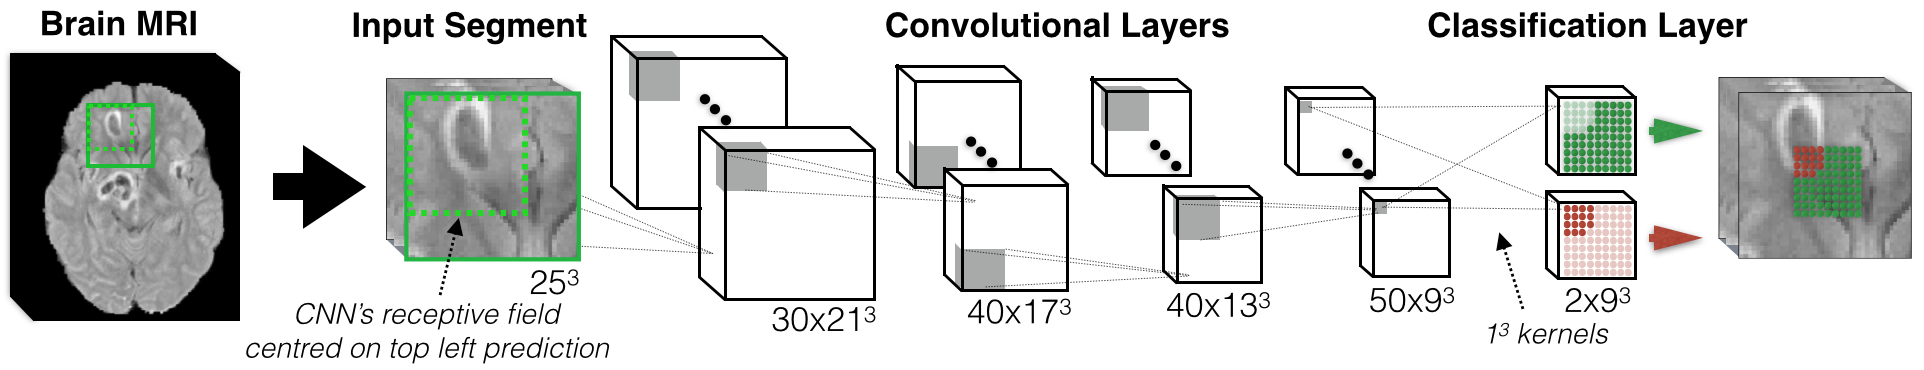
\includegraphics[clip=true, trim=0pt 0pt 0pt 0pt, width=1.0\textwidth]{figures/methodSection/cnnSystem/baselineDense.png}
\end{subfigure}
\fi
\caption{Our baseline CNN consists of four layers with $5^3$ kernels for feature extraction, leading to a receptive field of size $17^3$. The classification layer is implemented as convolutional with $1^3$ kernels, which enables efficient \textit{dense-inference}. When the network segments an input it predicts multiple voxels simultaneously, one for each shift of its receptive field over the input. Number of FMs and their size depicted as (\textit{Number $\times$ Size}).}
\label{fig:cnnBaseline}
\end{figure}


The neighborhood of voxels in the input that influence the activation of a neuron is its \textit{receptive field}. Its size, $\boldsymbol{\varphi}_l$, increases at each subsequent layer $l$ and is given by the 3-dimensional vector: 
\begin{equation} \label{eq:receptiveFile}
\boldsymbol{\varphi}_l^{\{ x,y,z\}} = \boldsymbol{\varphi}_{l-1}^{\{ x,y,z\}} + (\boldsymbol{\kappa}_l^{\{ x,y,z\}}-1) \boldsymbol{\tau}_l^{\{ x,y,z\}} \eqcm
\end{equation}
where $\boldsymbol{\kappa}_l,\boldsymbol{\tau}_l \in \mathbb{N}^3$ are vectors expressing the size of the kernels and stride of the receptive field at layer $l$. $\boldsymbol{\tau}_l$ is given by the product of the strides of kernels in layers preceding $l$. In this work only unary strides are used, as larger strides downsample the FMs (\cite{Springenberg2015}), which is unwanted behaviour for accurate segmentation. Thus in our system $\boldsymbol{\tau}_l = (1,1,1)$. The receptive field of a neuron in the classification layer corresponds to the image patch that influences the prediction for its central voxel. This is called the \textit{CNN's receptive field}, with $\boldsymbol{\varphi}_{CNN}=\boldsymbol{\varphi}_{L}$.

If input of size $\boldsymbol{\delta}_{in}$ is provided, the dimensions of the FMs in layer $l$ are given by:
\begin{equation} \label{eq:fmSize}
\boldsymbol{\delta}_l^{\{ x,y,z\}} = \lfloor (\boldsymbol{\delta}_{in}^{\{ x,y,z\}} - \boldsymbol{\varphi}_l^{\{ x,y,z\}}) / \boldsymbol{\tau}_l^{\{ x,y,z\}}	 +1 \rfloor
\end{equation}

In the common patch-wise classification setting, an input patch of size $\boldsymbol{\delta}_{in} = \boldsymbol{\varphi}_{CNN}$ is provided and the network outputs a single prediction for its central voxel. In this case the classification layer consists of FMs with size $1^3$. Networks that are implemented as fully-convolutionals are capable of \textit{dense-inference}, which is performed when input of size greater than $\boldsymbol{\varphi}_{CNN}$ is provided (\cite{Sermanet2013}). In this case, the dimensions of FMs increase according to Eq.~(\ref{eq:fmSize}). This includes the classification FMs which then output multiple predictions simultaneously, one for each stride of the CNN's receptive field on the input (Fig.~\ref{fig:cnnBaseline}). All predictions are equally trustworthy, as long as the receptive field is fully contained within the input and captures only original content, i.e. no padding is used. This strategy significantly reduces the computational costs and memory loads since the otherwise repeated computations of convolutions on the same voxels in overlapping patches are avoided. Optimal performance is achieved if the whole image is scanned in one forward pass. If GPU memory constraints do not allow it, such as in the case of large 3D networks where a large number of FMs need to be cached, the volume is tiled in multiple \textit{image-segments}, which are larger than individual patches, but small enough to fit into memory.

Before analyzing how we exploit the above dense-inference technique for training, which is the first main contribution of our work, we present the commonly used setting in which CNNs are trained patch-by-patch. Random patches of size $\boldsymbol{\varphi}_{CNN}$ are extracted from the training images. A \textit{batch} is formed out of $B$ of these samples, which is then processed by the network for one training iteration of Stochastic Gradient Descent (SGD). This step aims to alter the network's parameters $\mathbf{\Theta}$, such as weights and biases, in order to maximize the log likelihood of the data or, equally, minimize the Cross Entropy via the cost function:

\begin{equation} \label{eq:regCost}
J(\mathbf{\Theta}; \mathbf{I}^i, c^i)  = - \frac{1}{B} \sum_{i=1}^{B} \log\left(P(Y = c^i | \mathbf{I}^i, \mathbf{\Theta})\right) = - \frac{1}{B} \sum_{i=1}^{B} \log(p_{c^i}) \eqcm
\end{equation}
where the pair $(\mathbf{I}^i, c^i), \forall{i}\in{[1,B]}$ is the $i$-th patch in the batch and the true label of its central voxel, while the scalar value $p_{c^i}$ is the predicted posterior for class $c^i$. Regularization terms were omitted for simplicity. Multiple sequential optimization steps over different batches gradually lead to convergence.

\subsection{Dense Training on Image Segments and Class Balance}
\label{subsec:denseTraining}

Larger training batch sizes $B$ are preferred as they approximate the overall data more accurately and lead to better estimation of the true gradient by SGD. However, the memory requirement and computation time increase with the batch size. This limitation is especially relevant for 3D CNNs, where only a few dozens of patches can be processed within reasonable time on modern GPUs.

To overcome this problem, we devise a training strategy that exploits the dense inference technique on image segments. Following from Eq.~(\ref{eq:fmSize}), if an image segment of size greater than $\boldsymbol{\varphi}_{CNN}$ is given as input to our network, the output is a posterior probability for multiple voxels $V=\prod_{i=\{x,y,z\}}{\boldsymbol{\delta}_L^{(i)}}$. If the training batches are formed of $B$ segments extracted from the training images, the cost function (\ref{eq:regCost}) in the case of \textit{dense-training} becomes:

\begin{equation} \label{eq:costDense}
J_D(\mathbf{\Theta}; \mathbf{I}_s, \mathbf{c}_s) = - \frac{1}{B \cdot V} \sum_{s=1}^{B} \sum_{v=1}^{V} \log( p_{c_s^v}(\mathbf{x}^v)) \eqcm
\end{equation}

where $\mathbf{I}_s$ and $\mathbf{c}_s$ are the $s$-th segment of the batch and the true labels of its $V$ predicted voxels respectively. $c_s^v$ is the true label of the $v$-th voxel, $\mathbf{x}^v$ the corresponding position in the classification FMs and $p_{c_s^v}$ the output of the softmax function. The effective batch size is increased by a factor of $V$ without a corresponding increase in computational and memory requirements, as earlier discussed in Sec.~\ref{subsec:theBaseline}. Notice that this is a hybrid scheme between the commonly used training on individual patches and the dense training scheme on a whole image (\cite{Long2014}), with the latter being problematic to apply for training large 3D CNNs on volumes of high resolution due to memory limitations.



%+210 to left and -210 to right if I want to move one subfigure.

\begin{figure}[!h]
%\vspace{-1pt} %takes away some white space before figure
\centering
\begin{subfigure}[b]{0.5\textwidth}
\centering
	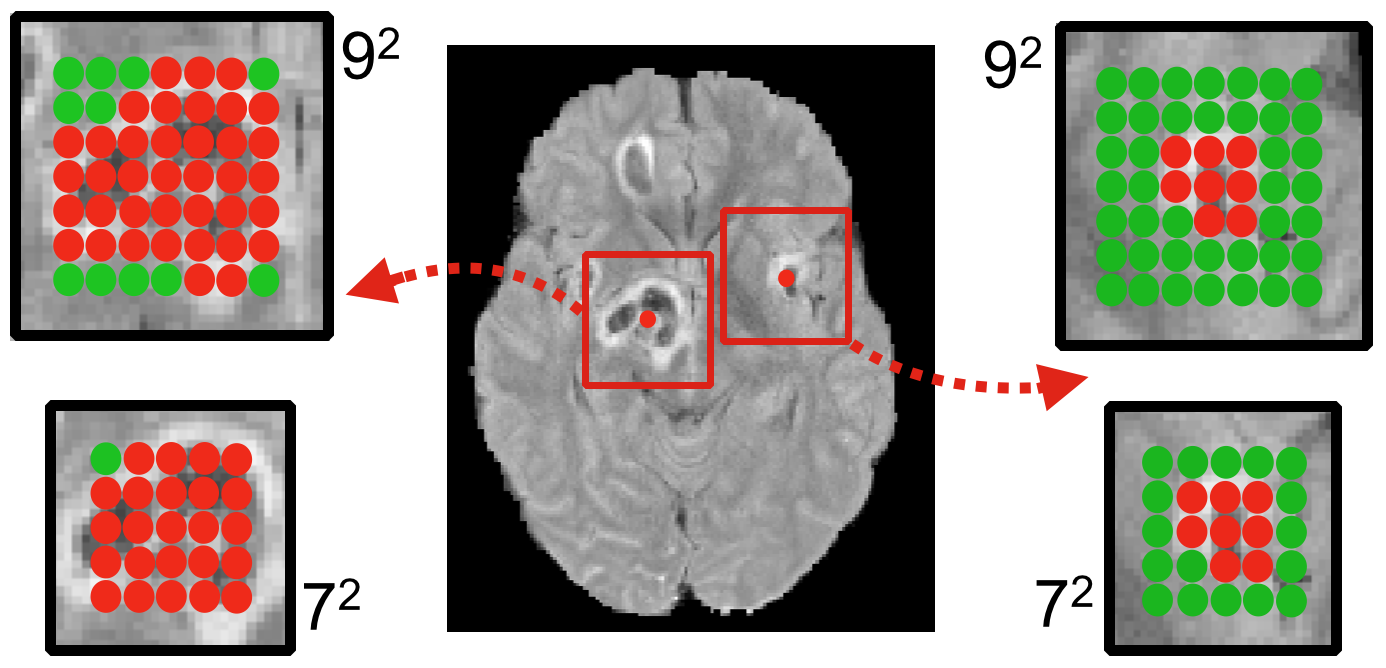
\includegraphics[clip=true, trim=0pt 0pt 0pt 0pt, width=1.0\textwidth]{figures/methodSection/denseTraining/segmentsVisual.png}
\end{subfigure}

\caption{Consider a network with a 2D receptive field of $3^2$ (for illustration) densely-applied on the depicted lesion-centred image segments of size $7^2$ or $9^2$. Relatively more background (green) is captured by larger segments and around smaller lesions.}
\label{fig:segmentsVisual}
\end{figure}

An appealing consequence of this scheme is that the sampling of input segments provides a flexible and automatic way to balance the distribution of training samples from different segmentation classes which is an important issue that directly impacts the segmentation accuracy. Specifically, we build the training batches by extracting segments from the training images with 50\% probability being centred on a foreground or background voxel, alleviating class-imbalance. Note that the predicted voxels $V$ in a segment do not have to be of the same class, something that occurs when a segment is sampled from a region near class boundaries (Fig.~\ref{fig:segmentsVisual}). Hence, the sampling rate of the proposed hybrid method adjusts to the true distribution of the segmentation task's classes. Specifically, the smaller a labelled object, the more background voxels will be captured within segments centred on the foreground voxel. Implicitly, this yields a balance between sensitivity and specificity in the case of binary segmentation tasks. In multi-class problems, the rate at which different classes are captured within a segment centred on foreground reflects the real relative distribution of the foreground classes, while adjusting their frequency relatively to the background.

\subsection{Building Deeper Networks}
\label{subsec:buildingADeeperNetwork}
Deeper networks have greater discriminative power due to the additional non-linearities and better quality of local optima (\cite{Choromanska2015}). However, convolutions with 3D kernels are computationally expensive in comparison to the 2D variants, which hampers the addition of more layers. Additionally, 3D architectures have a larger number of trainable parameters, with each layer adding $C_l C_{l-1} \prod_{i=\{x,y,z\}}{\boldsymbol{\kappa}_{l}^{(i)}}$ weights to the model. $C_l$ is the number of FMs in layer $l$ and $\boldsymbol{\kappa}_{l}^{\{x,y,z\}}$ the size of its kernel in the respective spatial dimension. Overall this makes the network increasingly prone to over-fitting.

In order to build a deeper 3D architecture, we adopt the sole use of small $3^3$ kernels that are faster to convolve with and contain less weights. This design approach was previously found beneficial for classification of natural images (\cite{Simonyan2014}) but its effect is even more drastic on 3D networks. When compared to common kernel choices of $5^3$ (\cite{zikic2014CnnBrats, urban2014CnnBrats, prasoon2013Knee}) and in our baseline CNN, the smaller $3^3$ kernels reduce the element-wise multiplications by a factor of approximately $5^3/3^3 \approx 4.6$ while reducing the number of trainable parameters by the same factor. Thus deeper network variants that are implicitly regularised and more efficient can be designed by simply replacing each layer of common architectures with more layers that use smaller kernels (Fig.~\ref{fig:deeper3x3}). 

%+210 to left and -210 to right if I want to move one subfigure.

\begin{figure}[!h]
%\vspace{-1pt} %takes away some white space before figure
\centering
\begin{subfigure}[b]{0.5\textwidth}
%subtracted 30pts from left and 80pts from the right. So also subtract 30/840 + 80/840 from the textwidth that whole should occupy to keep it correct scale. (23pts and 225pts original)
\centering
	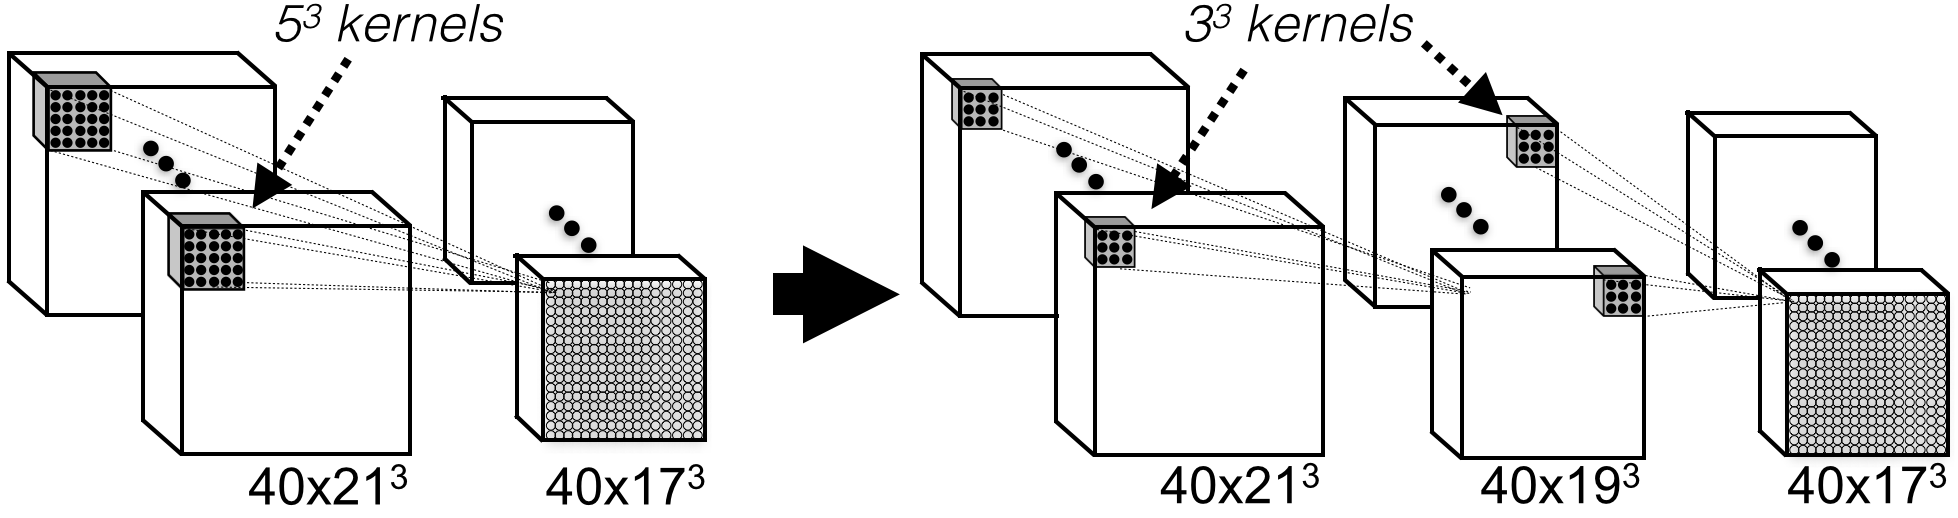
\includegraphics[clip=true, trim=0pt 0pt 0pt 0pt, width=1.0\textwidth]{figures/methodSection/deepProblems/deeper3x3.png}
\end{subfigure}

\caption{The replacement of the depicted layer with $5^5$ kernels (left) with two successive layers using $3^3$ kernels (right) introduces an additional non-linearity without altering the CNN's receptive field. Additionally, the number of weights is reduced from 200k to 86.4k and the required convolutions are cheaper (see text). Number of FMs and their size depicted as (\textit{Number $\times$ Size}).}
\label{fig:deeper3x3}
\end{figure}
%\vspace{-1pt} %takes away some white space before figure



However, deeper networks are more difficult to train. It has been shown that the forward (neuron activations) and backwards (gradients) propagated signal may explode or vanish if care is not given to retain its variance (\cite{Glorot2010}). This occurs because at every successive layer $l$, the variance of the signal is multiplied by $n^{in}_l \cdot var(\mathbf{W}_l)$, where $n^{in}_l=C_{l-1} \prod_{i=\{x,y,z\}}{\boldsymbol{\kappa}_{l}^{(i)}}$ is the number of weights through which a neuron of layer $l$ is connected to its input and $var(\mathbf{W}_l)$ is the variance of the layer's weights. To better preserve the signal in the initial training stage we adopt a scheme recently derived for ReLu-based networks by \cite{he2015delving} and initialize the kernel weights of our system by sampling from the normal distribution $\mathcal{N}(0,\sqrt{2/n^{in}_l})$.

A phenomenon of similar nature that hinders the network's performance is the \quot{internal covariate shift} (\cite{ioffe2015batch}). It occurs throughout training, because the weight updates to deeper layers result in a continuously changing distribution of signal at higher layers, which hinders the convergence of their weights. Specifically, at training iteration $t$ the weight updates may cause deviation $\epsilon_{l,t}$ to the variance of the weights. At the next iteration the signal will be amplified by $n^{in}_l \cdot var(\mathbf{W}_{l,t+1}) = n^{in}_l \cdot (var(\mathbf{W}_{l,t}) + \epsilon_{l,t})$. Thus before influencing the signal, any deviation $\epsilon_{l,t}$ is amplified by $n^{in}_l$ which is exponential in the number of dimensions. For this reason the problem affects training of 3D CNNs more severely than conventional 2D systems. For countering it, we adopt the recently proposed Batch Normalisation (BN) technique to all hidden layers (\cite{ioffe2015batch}), which allows normalization of the FM activations at every optimization step in order to better preserve the signal.


\subsection{Multi-Scale Processing via Parallel Convolutional Pathways}
\label{subsec:multiscaleCnn}

The segmentation of each voxel is performed by taking into account the contextual information that is captured by the receptive field of the CNN when it is centred on the voxel. The spatial context is providing important information for being able to discriminate voxels that otherwise appear very similar when considering only local appearance. From Eq.~(\ref{eq:receptiveFile}) follows that an increase of the CNN's receptive field requires bigger kernels or more convolutional layers, which increases computation and memory requirements. An alternative would be the use of pooling (\cite{LeCun1998}), which however leads to loss of the exact position of the segmented voxel and thus can negatively impact accuracy.

In order to incorporate both local and larger contextual information into our 3D CNN, we add a second pathway that operates on down-sampled images. Thus, our dual pathway 3D CNN simultaneously processes the input image at multiple scales (Fig.~\ref{fig:cnnMultiscale}). Higher level features such as the location within the brain are learned in the second pathway, while the detailed local appearance of structures is captured in the first. As the two pathways are decoupled in this architecture, arbitrarily large context can be processed by the second pathway by simply adjusting the down-sampling factor $F_D$. The size of the pathways can be independently adjusted according to the computational capacity and the task at hand, which may require relatively more or less filters focused on the down-sampled context.

%+210 to left and -210 to right if I want to move one subfigure.

\begin{figure}[!h]
%\vspace{-1pt} %takes away some white space before figure
\centering
\begin{subfigure}[b]{1.0\textwidth}
\centering
	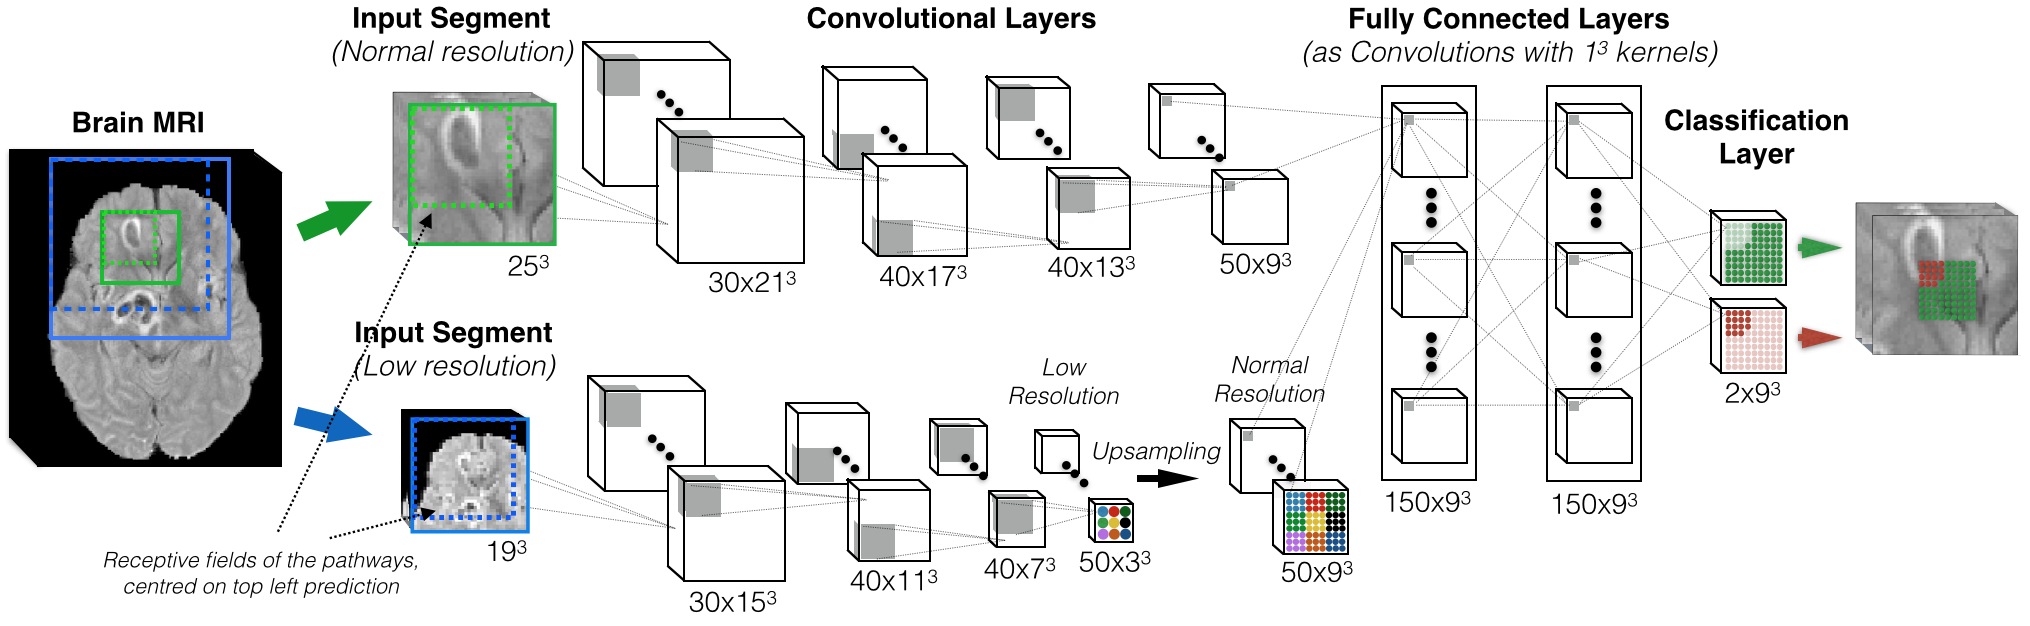
\includegraphics[clip=true, trim=0pt 0pt 0pt 0pt, width=1.0\textwidth]{figures/methodSection/multiscale/cnnSystemMultiscale.png}
\end{subfigure}
\caption{Multi-scale 3D CNN with two convolutional pathways. The kernels of the two pathways are here of size $5^3$ (for illustration only to reduce the number of layers in the figure). The neurons of the last layers of the two pathways thus have receptive fields of size $17^3$ voxels. The inputs of the two pathways are centered at the same image location, but the second segment is extracted from a down-sampled version of the image by a factor of 3. The second pathway processes context in an actual area of size $51^3$ voxels. \textit{DeepMedic}, our proposed 11-layers architecture, results by replacing each layer of the depicted pathways with two that use $3^3$ kernels (see Sec.~\ref{subsec:buildingADeeperNetwork}). Number of FMs and their size depicted as (\textit{Number $\times$ Size}).}
\label{fig:cnnMultiscale}
\end{figure}
%\vspace{-1pt} %takes away some white space before figure

To preserve the capability of dense inference, spatial correspondence of the activations in the FMs of the last convolutional layers of the two pathways, $L1$ and $L2$, should be ensured. In networks  where only unary kernel strides are used, such as the proposed architecture, this requires that for every $F_D$ shifts of the receptive field $\boldsymbol{\varphi}_{L1}$ over the normal resolution input, only one shift is performed by $\boldsymbol{\varphi}_{L2}$ over the down-sampled input. Hence it is required that the dimensions of the FMs in $L2$ are $\boldsymbol{\delta}_{L2}^{\{ x,y,z\}} = \lceil \boldsymbol{\delta}_{L1}^{\{ x,y,z\}} / F_D \rceil$. From Eq.~(\ref{eq:fmSize}), the size of the input to the second pathway is $\boldsymbol{\delta}_{in2}^{\{ x,y,z\}} = \boldsymbol{\varphi}_{L2}^{\{ x,y,z\}} + \boldsymbol{\delta}_{L2}^{\{ x,y,z\}} -1 $ and similar is the relation between $\boldsymbol{\delta}_{in1}$ and $\boldsymbol{\delta}_{L1}$. These establish the relation between the required dimensions of the input segments from the two resolutions, which can then be extracted centered on the same image location. The FMs of $L2$ are up-sampled to match the dimensions of $L1$'s FMs and are then concatenated together. We add two more hidden layers for combining the multi-scale features before the final classification, as shown in Fig.~\ref{fig:cnnMultiscale}. Integration of the multi-scale parallel pathways in architectures with non-unary strides is discussed in \ref{app:detailsMultiscale}.

Combining multi-scale features has been found beneficial in other recent works (\cite{Long2014, Ronneberger2015}), in which whole 2D images are processed in the network by applying a few number of convolutions and then down-sampling the FMs for further processing at various scales. Our decoupled pathways allow arbitrarily large context to be provided while avoiding the need to load large parts of the 3D volume into memory. Additionally, our architecture extracts features completely independently from the multiple resolutions. This way, the features learned by the first pathway retain finest details, as they are not involved in processing low resolution context.

\subsection{3D Fully Connected CRF for Structured Prediction}
\label{subsec:3dFcCrf}

Because neighboring voxels share substantial spatial context, the soft segmentation maps produced by the CNN tend to be smooth, even though neighborhood dependencies are not modeled directly. However, local minima in training and noise in the input images can still result in some spurious outputs, with small isolated regions or holes in the predictions. We employ a fully connected CRF (\cite{Krahenbuhl2013}) as a post-processing step to achieve more structured predictions. As we describe below, this CRF is capable of modeling arbitrarily large voxel-neighborhoods but is also computationally efficient, making it ideal for processing 3D multi-modal medical scans.

For an input image $\mathbf{I}$ and the label configuration (segmentation) $\mathbf{z}$, the Gibbs energy in a CRF model is given by

\begin{equation}
E(\mathbf{z}) = \sum_i{\psi_u(z_i)} + \sum_{ij, i \neq j}{\psi_p(z_i,z_j)} \eqfs
\end{equation}

The unary potential is the negative log-likelihood $\psi_u(z_i) = -logP(z_i|\mathbf{I})$, where in our case $P(z_i|\mathbf{I})$ is the CNN's output for voxel $i$. In a fully connected CRF, the pairwise potential is of form $\psi_p(z_i,z_j) = \mu(z_i,z_j) k(\mathbf{f_i},\mathbf{f_j})$ between any pair of voxels, regardless of their spatial distance. The Pott's Model is commonly used as the label compatibility function, giving $\mu(z_i,z_j)=[z_i \neq z_j]$. The corresponding energy penalty is given by the function $k$, which is defined over an arbitrary feature space, with $\mathbf{f_i},\mathbf{f_j}$ being the feature vectors of the pair of voxels. \cite{Krahenbuhl2013} observed that if the penalty function is defined as a linear combination of Gaussian kernels, $k(\mathbf{f_i},\mathbf{f_j}) = \sum_{m=1}^{M} {w^{(m)}k^{(m)}(\mathbf{f_i},\mathbf{f_j})}$, the model lends itself for very efficient inference with mean field approximation, after expressing message passing as convolutions with the Gaussian kernels in the space of the feature vectors $\mathbf{f_i},\mathbf{f_j}$.

We extended the work of the original authors and implemented a 3D version of the CRF for processing multi-modal scans. We make use of two Gaussian kernels, which operate in the feature space defined by the voxel coordinates $p_{i,d}$ and the intensities of the $c$-th modality-channel $I_{i,c}$ for voxel $i$. The smoothness kernel, $k^{(1)}(\mathbf{f_i}, \mathbf{f_j}) = exp\Big(- \sum_{d=\{x,y,z\}}{ \frac{\vert p_{i,d} - p_{j,d} \vert ^2}{2\sigma_{\alpha, d}^2} } \Big)$, is defined by a diagonal covariance matrix with elements the configurable parameters $\sigma_{\alpha, d}$, one for each axis. These parameters express the size and shape of neighborhoods that homogeneous labels are encouraged. The appearance kernel $ k^{(2)}(\mathbf{f_i},\mathbf{f_j}) = exp \Big( - \sum_{d=\{x,y,z\}}{ \frac{\vert p_{i,d}-p_{j,d} \vert ^2}{2\sigma_{\beta,d}^2} } - \sum_{c=1}^{C}{ \frac{\vert I_{i,c} - I_{j,c} \vert ^2}{2\sigma_{\gamma,c}^2} } \Big) $ is defined similarly. The additional parameters $\sigma_{\gamma,c}$ can be interpreted as how strongly to enforce homogeneous appearance in the $C$ input channels, when voxels in an area spatially defined by $\sigma_{\beta,d}$ are identically labelled. Finally, the configurable weights $w^{(1)},w^{(2)}$ define the relative strength of the two factors.

